\documentclass[border=0.15cm]{standalone}
\usepackage{tikz}
\usetikzlibrary{automata, arrows.meta, positioning}

\begin{document}
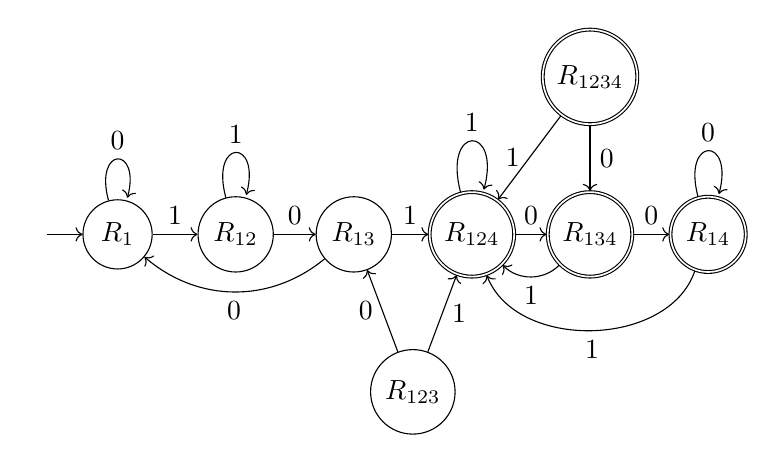
\begin{tikzpicture}
    every initial by arrow/.style = {-To},
    every loop/.style = {-To}]
    % \draw [help lines] (-1,-1) grid (5,1);
    \node (R1) [state, 
        initial, 
        initial text={}] at (0,0) {$R_{1}$};
    \node (R12) [state] at (1.5,0) {$R_{12}$};
    \node (R13) [state] at (3.0,0) {$R_{13}$};
    \node (R124) [state, accepting] at (4.5,0) {$R_{124}$};
    \node (R134) [state, accepting] at (6.0,0) {$R_{134}$};
    \node (R14) [state, accepting] at (7.5,0) {$R_{14}$};
    \node (R123) [state] at (3.75,-2.0) {$R_{123}$};
    \node (R1234) [state, accepting] at (6.0, 2.0) {$R_{1234}$};

    \path [-To]
        (R1) edge node [above] {$1$} (R12)
        (R12) edge node [above] {$0$} (R13)
        (R13) edge node [above] {$1$} (R124)
        (R13) edge [bend left=40] node [below] {$0$} (R1)
        (R124) edge node [above] {$0$} (R134)
        (R134) edge node [above] {$0$} (R14)
        (R134) edge [bend left=45] node [below] {$1$} (R124)
        (R14) edge [bend left=70] node [below] {$1$} (R124)
        (R123) edge node [left] {$0$} (R13)
        (R123) edge node [right] {$1$} (R124)
        (R1234) edge node [right] {$0$} (R134)
        (R1234) edge node [left] {$1$} (R124)
        (R1) edge [loop above] node {$0$} ()
        (R12) edge [loop above] node {$1$} ()
        (R124) edge [loop above] node {$1$} ()
        (R14) edge [loop above] node {$0$} ();
\end{tikzpicture}
\end{document}